\section{¿Qué es Git?}

. . .

\begin{itemize}
\item
  Git y GitHub no son la misma cosa
\item
  Git es un sistema de control de versiones
\item
  Permite organizar diferentes versiones de un mismo archivo o todo un
  proyecto
\item
  Permite colaborar con otras personas
\end{itemize}

\subsection{Qué es GitHub?}

\begin{itemize}
\item
  GitHub es un servicio de almacenamiento. Como Drive
\item
  Da otras cosas útiles como issues, pull requests, etc\ldots{}
\end{itemize}

\subsection{Meme ilustrativo}

\begin{figure}
\centering

\includegraphics{figs/meme_git_v_gh.jpg}
\caption{Meme ilustrativo.}
\end{figure}

\section{Cómo funciona Git?}

\subsection{Analogía con Roma}

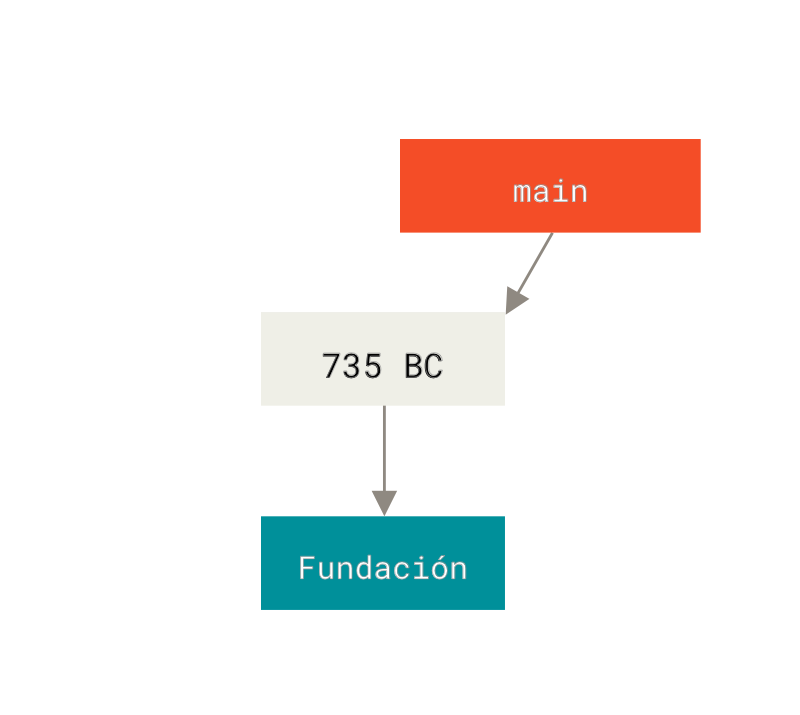
\includegraphics{figs/stage1.png}

\subsection{Julio Cesar se vuelve emperador}

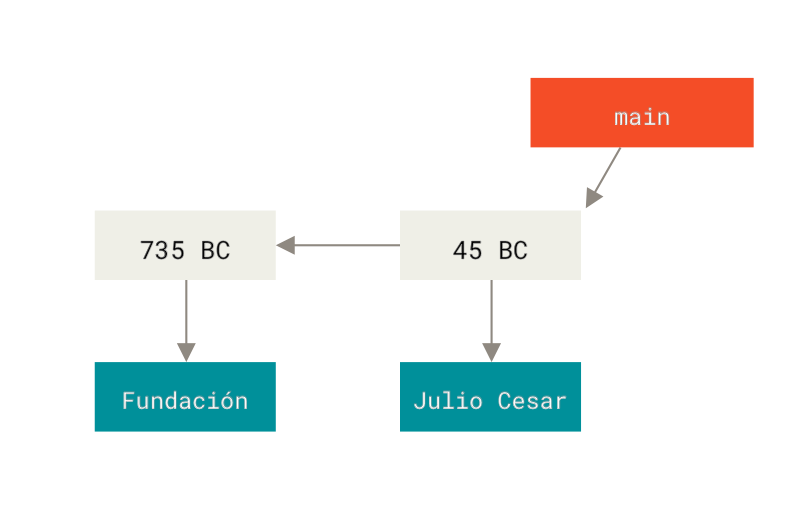
\includegraphics{figs/stage2.png}

\subsection{Brutus asesina a Julio Cesar}

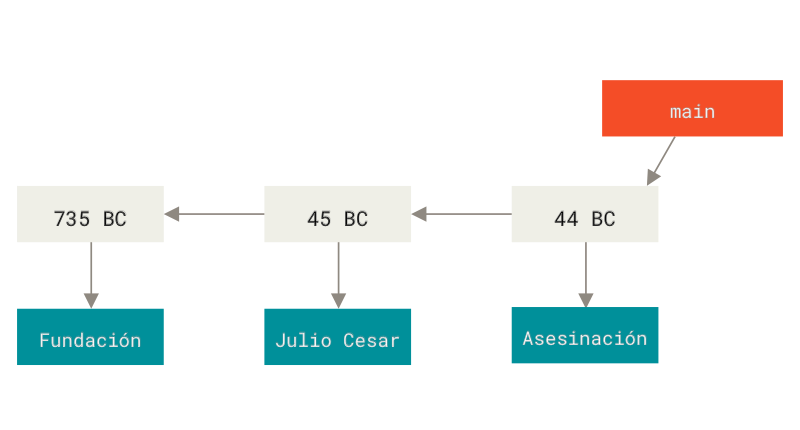
\includegraphics{figs/stage3.png}

\subsection{Bifurcación}

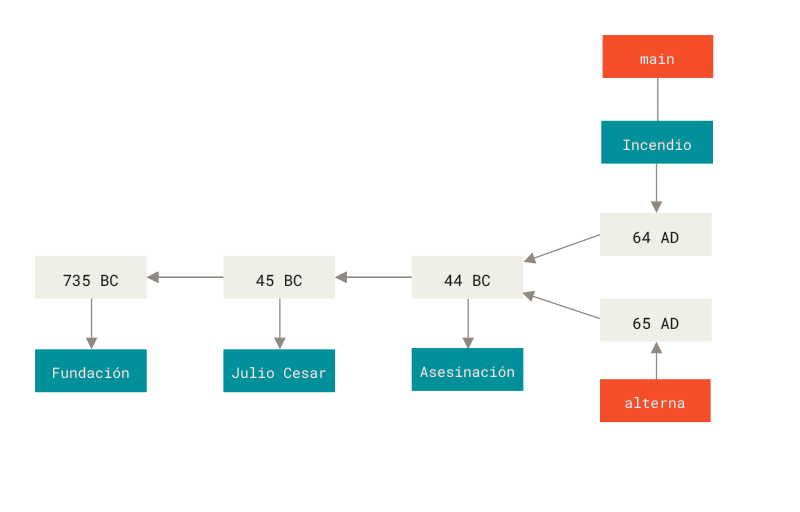
\includegraphics{figs/stage4.png}

\subsection{Modelo distribuido}

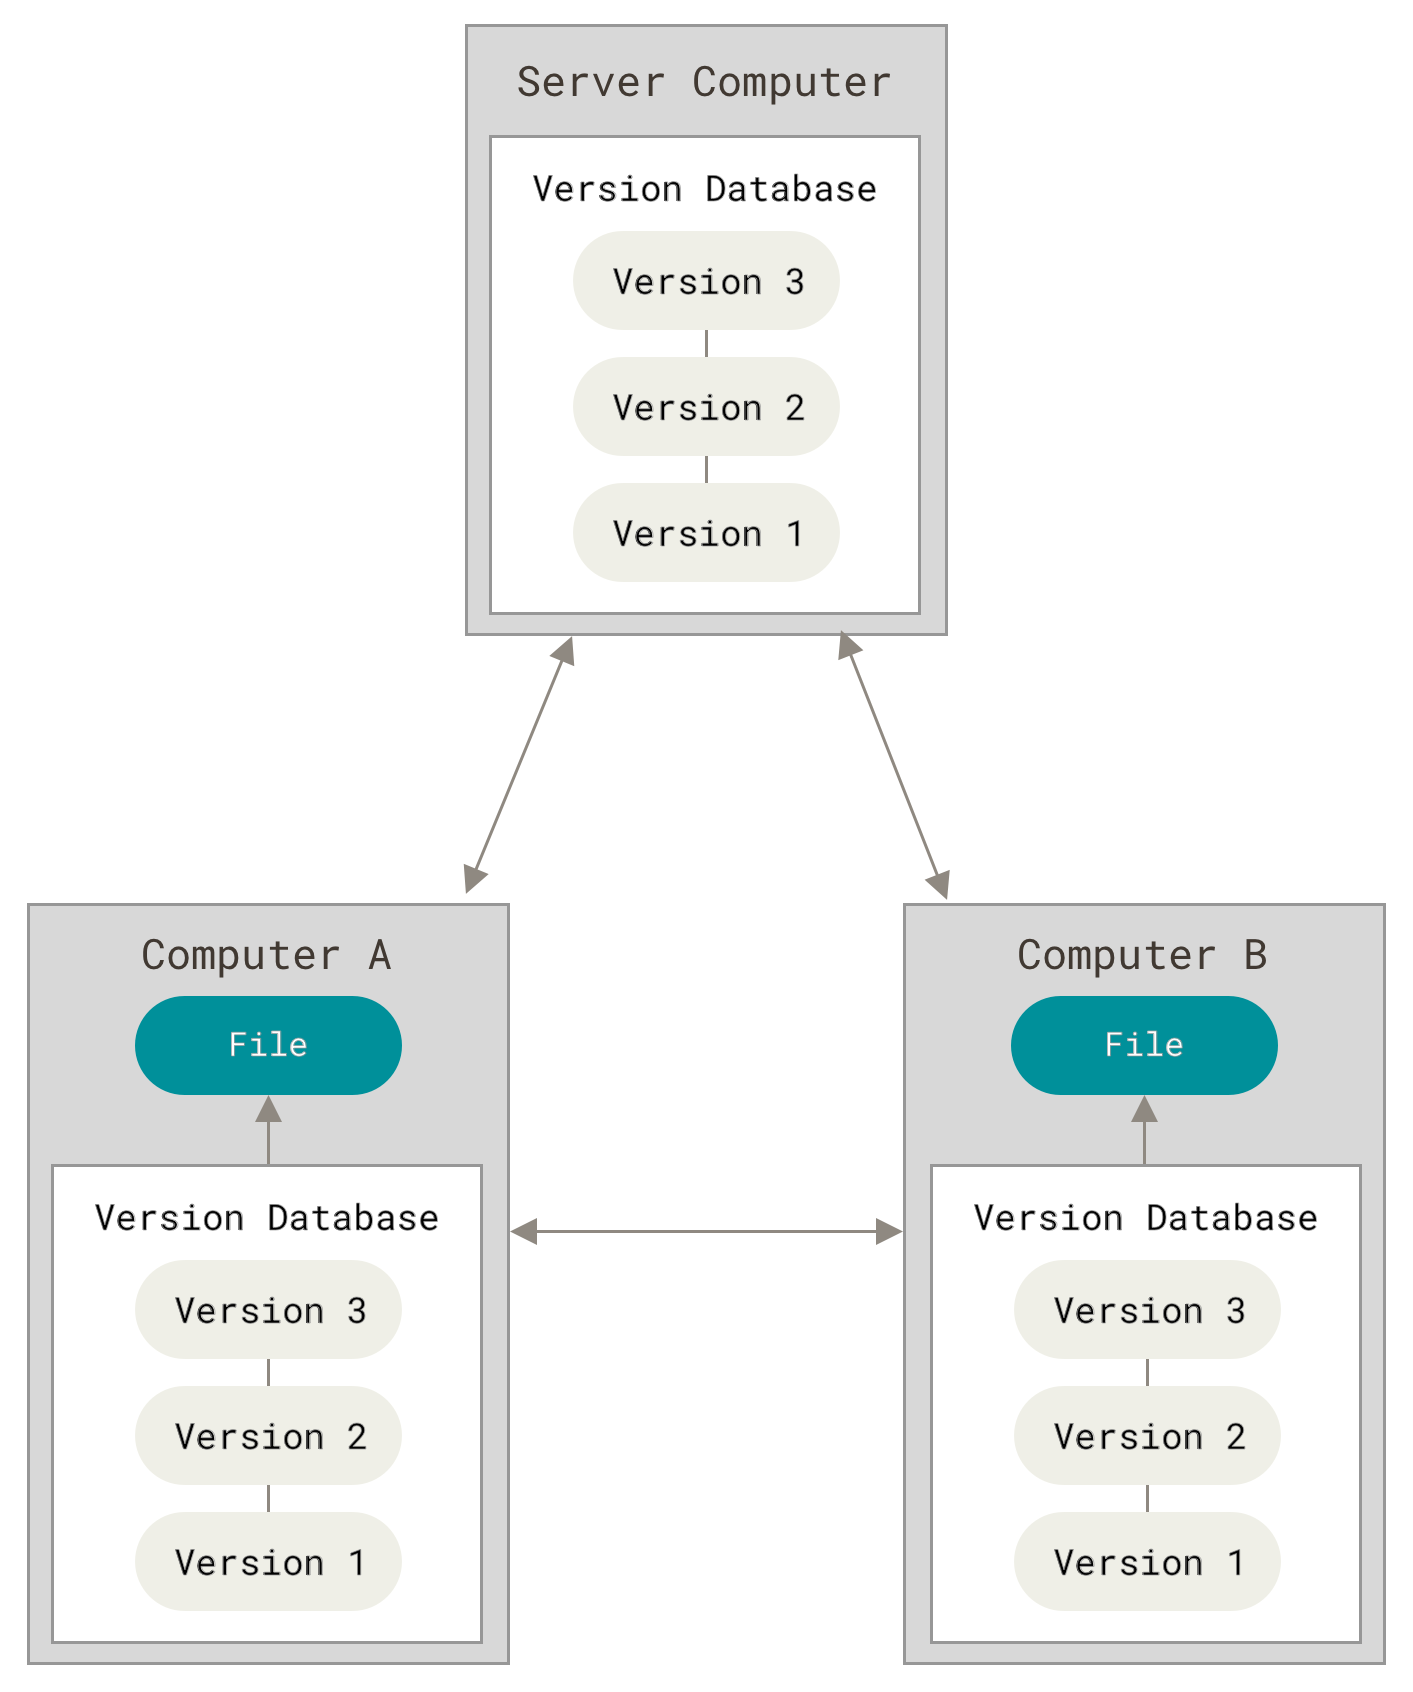
\includegraphics{figs/distributed.png} \# The Three States Git tiene
tres estados en los que puede estar un archivo en cualquier momento
dado:

\begin{itemize}
\item
  \textbf{Modified}
\item
  \textbf{Staged / Preparado}
\item
  \textbf{Committed / Confirmado}
\end{itemize}

. . .

\begin{enumerate}
\def\labelenumi{\arabic{enumi}.}
\tightlist
\item
  Ignorados
\end{enumerate}

\subsection{Tres etapas}

Similarmente, hay tres secciones o ``espacios'' en cada proyecto de Git:

\begin{enumerate}
\def\labelenumi{\arabic{enumi}.}
\item
  Working Directory.
\item
  Staging Area.
\item
  Git Repository.
\end{enumerate}

\section{Basic Git Workflow}

\begin{enumerate}
\def\labelenumi{\arabic{enumi}.}
\item
  Modifica archivos locales en disco.
\item
  Se elige qué archivos se desea rastrear (\emph{track}) añadiéndolos al
  \emph{staging area}.

  \begin{itemize}
  \tightlist
  \item
    Son estos y solo estos los archivos que serán parte del siguiente
    commit
  \end{itemize}
\item
  Se hace un \emph{commit} o confirmación

  \begin{itemize}
  \tightlist
  \item
    Esta versión queda guardada en el historial de cambios.
  \end{itemize}
\end{enumerate}

\section{Básicos de Git}

\section{Getting a Git Repository}

Usualmente uno obtiene un repositorio de Git en dos maneras:

\begin{enumerate}
\def\labelenumi{\arabic{enumi}.}
\item
  Se crea un repo con una carpeta existente, o bien.
\item
  \emph{Clonas} un repositorio de Git existente de algún otro lugar.
\end{enumerate}

\section{¿Cómo iniciar repo con carpeta existente?}

. . .

\subsection{Inicializando un repo vacío.}

\begin{lstlisting}[language=bash]
$ git init
\end{lstlisting}

. . .

Señalando qué archivos rastrear. En este caso todos los de python.

\begin{lstlisting}[language=bash]
$ git add *.py
\end{lstlisting}

\subsection{Notas}

\begin{quote}
El comando \passthrough{\lstinline!git add!} tiene dos funciones: Cambia
el estatus de un archivo de \emph{untracked} a \emph{tracked}, y además
añade archivos \emph{modified} al \emph{staging area} para prepararlos
para un \emph{commit}.

\passthrough{\lstinline!add!} recibe como argumento nombres de archivos,
o patrones \emph{glob}.
\end{quote}

\section{Obteniendo un repo de un lugar remoto}

Podemos hacer un \emph{clon} exacto de un proyecto con todo y su
historial de cambios.

\subsection{Clonando de algún lugar en internet}

Dado un URL:

. . .

\begin{lstlisting}
$ git clone https://github.com/progit/progit2
\end{lstlisting}

Esto crea una nueva carpeta en tu current working directory con los
archivos del repo \& el historial de cambios. \# Recording changes

Una vez que se tiene un repositorio de Git y archivos rastreados, se
puede empezar a usar todo el potencial de Git.

\subsection{Ciclo de vida de un archivo}

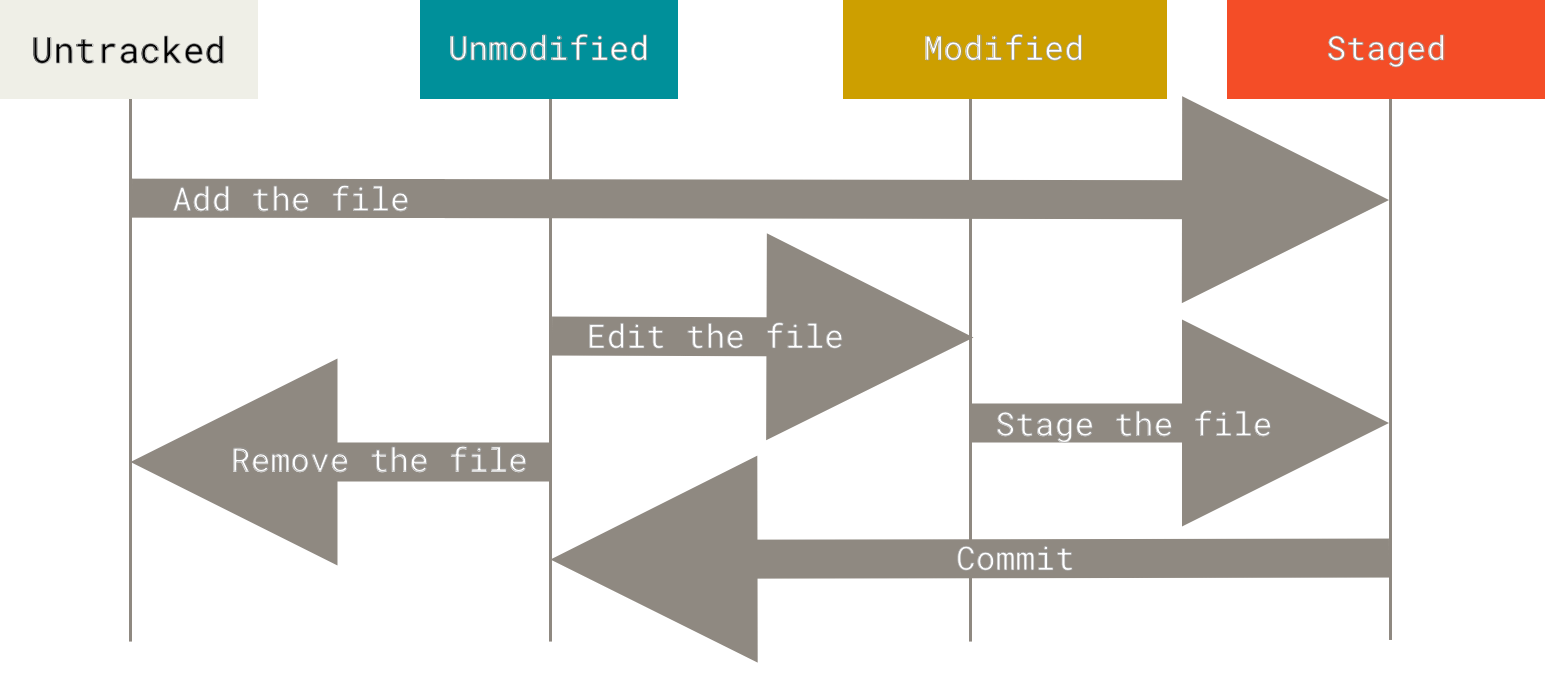
\includegraphics{figs/lifecycle.png}

. . .

Para checar en qué punto del ciclo se encuentran los archivos existe el
comando \passthrough{\lstinline!git status!}.

\subsection{Checando estatus}

\begin{itemize}
\item
  ``working directory clean'' significa que no hay cambios
\item
  Veamos qué pasa al añadir un archivo
\item
  Git reconoce el archivo, pero no rastreará sus cambios. Usamos\ldots{}
\item
  Un paso antes de confirmar
\end{itemize}

\section{Commiting your changes}

\begin{enumerate}
\def\labelenumi{\arabic{enumi}.}
\tightlist
\item
  Guardar cambios en git con: \passthrough{\lstinline!git commit!}.

  \begin{itemize}
  \tightlist
  \item
    Es mejor siempre usar el modificador \passthrough{\lstinline!-m!}
  \end{itemize}
\item
  El output da información interesante:

  \begin{itemize}
  \tightlist
  \item
    Nombre de rama. Aquí \passthrough{\lstinline!main!}.
  \item
    Código alfanumérico llamado checksum
  \item
    Estadísticas de cambios
  \end{itemize}
\end{enumerate}

\subsection{Un pequeño atajo}

Es común querer agregar todo lo modificado al staging area directamente.

. . .

Combinamos modificadores \passthrough{\lstinline!-m!} con
\passthrough{\lstinline!-a!} que es corto para
\passthrough{\lstinline!--all!}.

\begin{lstlisting}
$ git commit -a -m "Fixes"
\end{lstlisting}

\section{Compartiendo con el mundo}

El punto entero es trabajar con otras personas.

. . .

Recordamos el modelo distribuido anterior.

\subsection{}

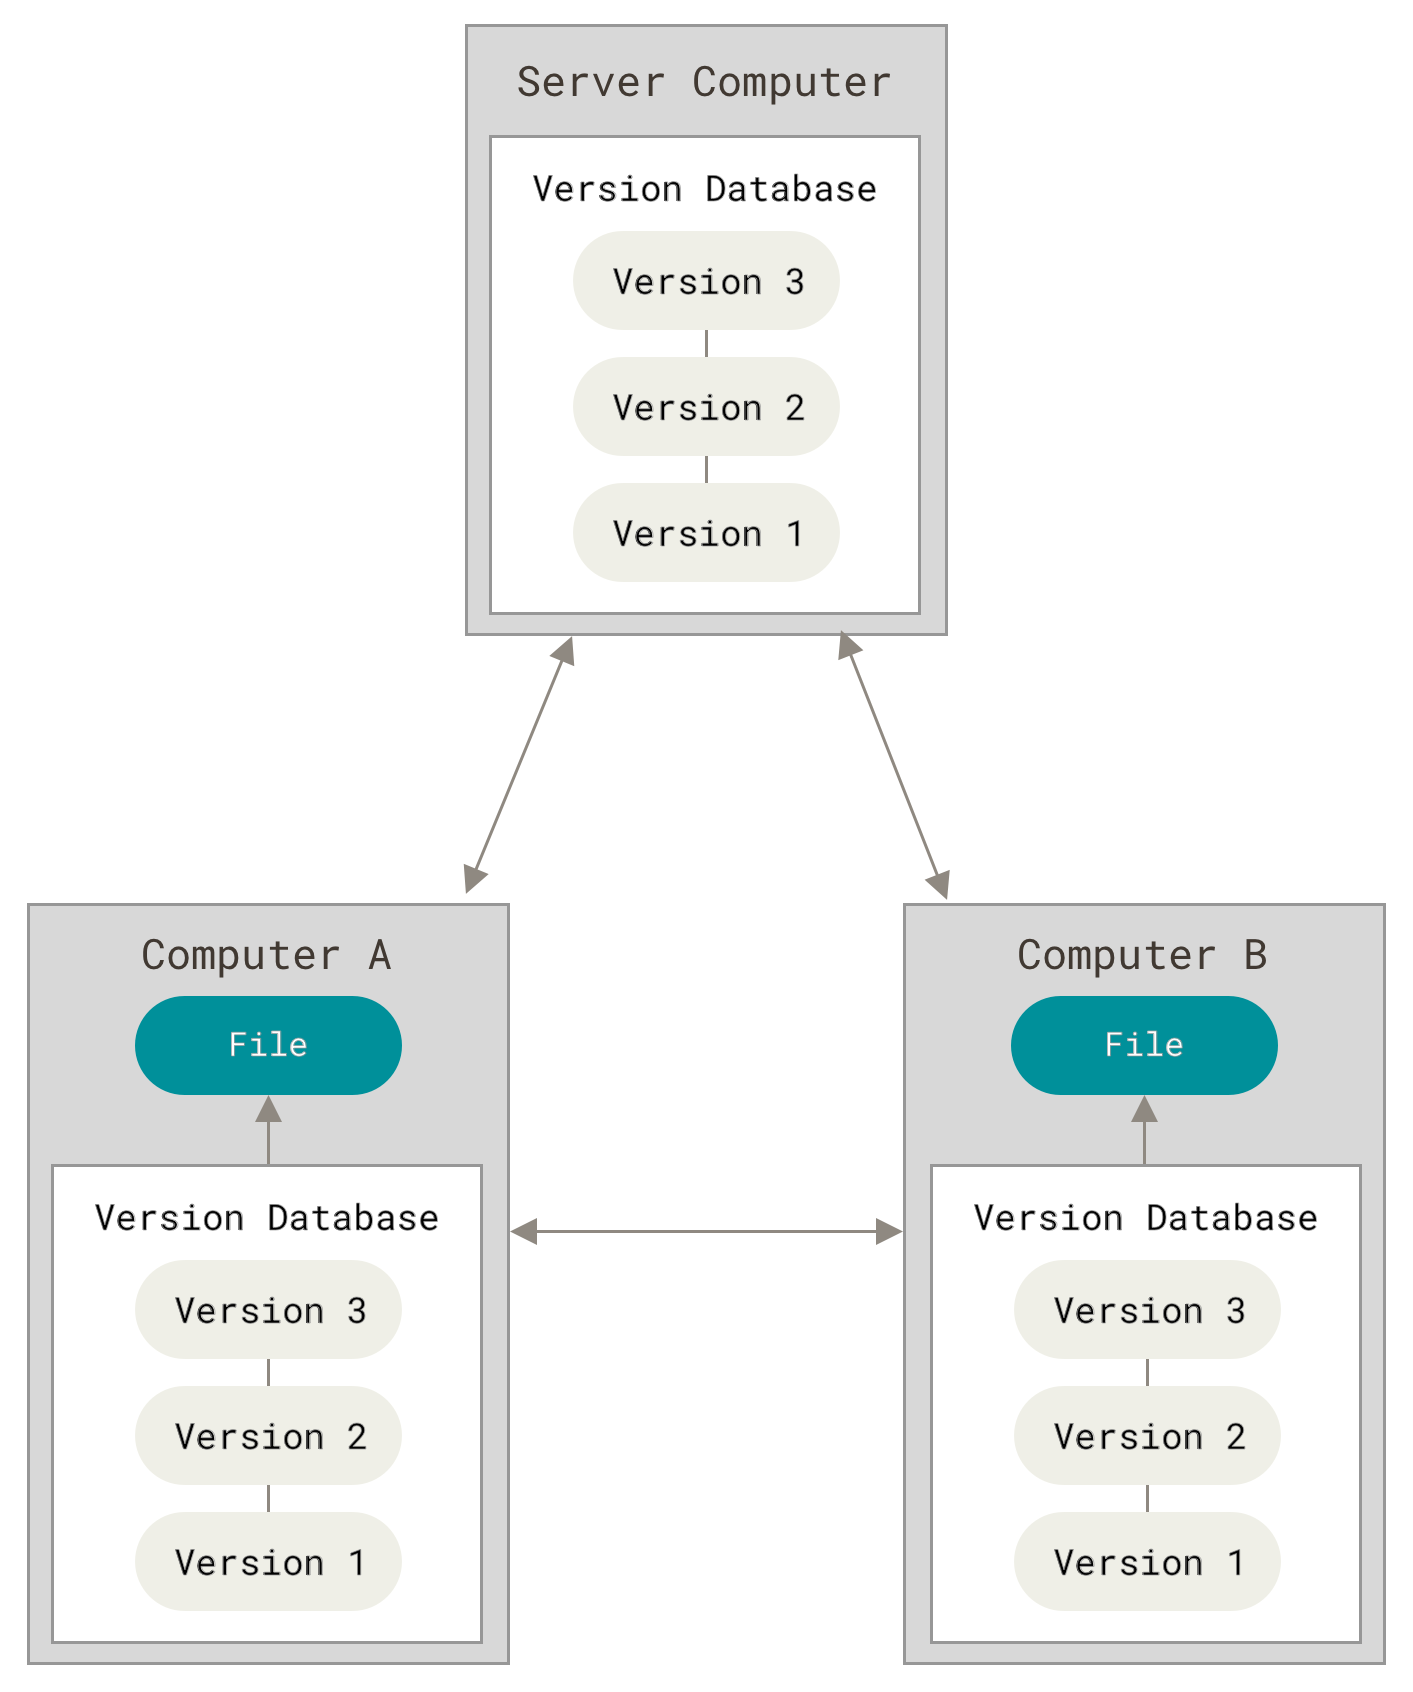
\includegraphics{figs/distributed.png}

. . .

En este caso GitHub será el remoto. (Server)

\subsection{}

El comando push se contacta con el remoto.

\begin{lstlisting}
$ git push origin main
\end{lstlisting}

. . .

Toma 2 cosas:

\begin{itemize}
\tightlist
\item
  El nombre del remoto: \passthrough{\lstinline!origin!}
\item
  El nombre de la ``rama'': \passthrough{\lstinline!main!} \# Viewing
  the Commit History
\end{itemize}

El punto entero de tener un sistema de control de versiones es poder
registrar cambios graduales

Para revisar el historial de cambios y confirmaciones existe el comando
\passthrough{\lstinline!git log!}. Vamos a correrlo.

\subsection{}

Muestra un listado de commits en orden cronológico inverso e información
relevante de cada uno.

Algunos modificadores útiles:

\begin{itemize}
\tightlist
\item
  \passthrough{\lstinline!-n!} para mostrar los \(n\) más recientes.
\item
  \passthrough{\lstinline!-p!} cambios hechos por cada commit.
\item
  \passthrough{\lstinline!-stat!} estadísticas descriptivas
\end{itemize}

\section{Undoing things}

De las cosas más útiles de usar git es que se pueden revertir cambios.
Algunos ejemplos prácticos

\subsection{Committeando antes de tiempo}

. . .

\begin{lstlisting}
$ git commit --ammend -m "Mensaje"
\end{lstlisting}

Permite por ejemplo cambiar mensaje de confirmación

\subsection{Staging antes de tiempo}

Para ``bajar'' un archivo del staging area

\begin{lstlisting}
$ git reset HEAD <archivo>
\end{lstlisting}

\subsection{Revertir un archivo al commit previo}

. . .

\begin{lstlisting}
$ git checkout - <archivo>
\end{lstlisting}

. . .

\begin{quote}
Precaución: No hay manera de revertir este cambio. Se reemplaza por
completo al archivo con otra versión distinta. \# Working with remotes
\end{quote}

Un remote es el servidor externo en el modelo distribuido.

. . .

Interactuamos con remotes a través de 3 comandos:

\begin{itemize}
\tightlist
\item
  \passthrough{\lstinline!pull!}
\item
  \passthrough{\lstinline!push!}
\item
  \passthrough{\lstinline!fech!}
\end{itemize}

\subsection{Listando remotes}

\begin{lstlisting}
$ git remote -v
\end{lstlisting}

. . .

Si se clonó de GitHub verás el URL original. Si se inició con una
carpeta no habrá ningún remote configurado

. . .

Cuando se clona un repo se añade automáticamente un remote:
\passthrough{\lstinline!origin!}.

. . .

Se pueden añadir remotes

\begin{lstlisting}
$ git remote add <shortname> <url>
\end{lstlisting}

\subsection{Pulling}

Podemos \emph{jalar} (descargar) la versión de una rama específica de un
remoto específico.

\begin{lstlisting}
$ git pull <remote> <branch>
\end{lstlisting}

Pull no solo baja los contenidos, sino que los \emph{mezcla} con la rama
actual

. . .

Se puede descargar sin mezclar con fetch.

\begin{lstlisting}
$ git fetch origin main
\end{lstlisting}

Que crea una \emph{rama} nueva sin modificar tus archivos.

\subsection{Pushing}

Se puede subir a GitHub con el comando \passthrough{\lstinline!push!}.

\begin{lstlisting}
$ git push <remote> <branch>
\end{lstlisting}

. . .

Para poder hacer push debes estar al día con
\passthrough{\lstinline!<branch>!}

. . .

Más información de un remote con

\begin{lstlisting}
$ git remote show <remote>
\end{lstlisting}

\subsection{Tagging}

Otra habilidad de Git es etiquetar (\emph{tag}) \emph{commit}s
específicos

Permite ir clasificando por ``versiones'', como 1.0.x

. . .

Se listan los tags existentes con \passthrough{\lstinline!git tag!}. \#
Git Branching

Las ramas permiten bifurcar el árbol de versiones.

\subsection{}

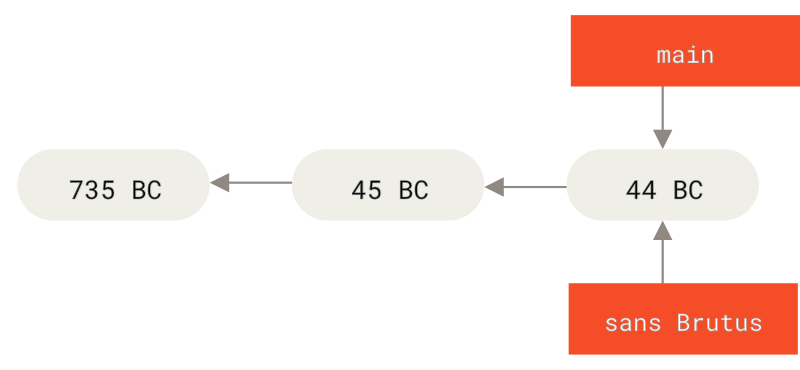
\includegraphics{figs/timeline1.png}

\subsection{}

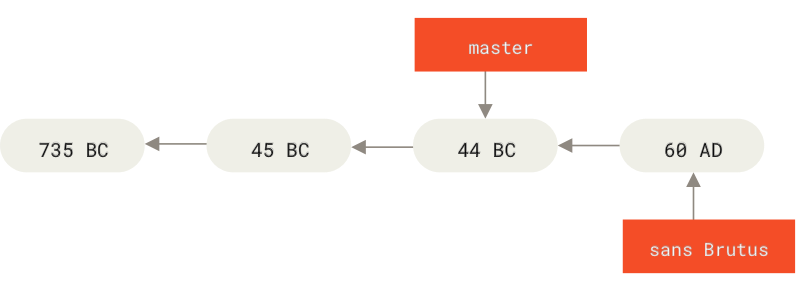
\includegraphics{figs/timeline2.png}

\subsection{}

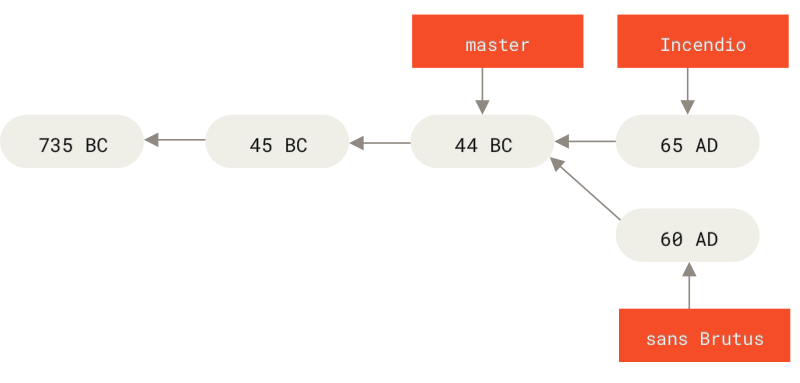
\includegraphics{figs/timeline3.png}

\subsection{}

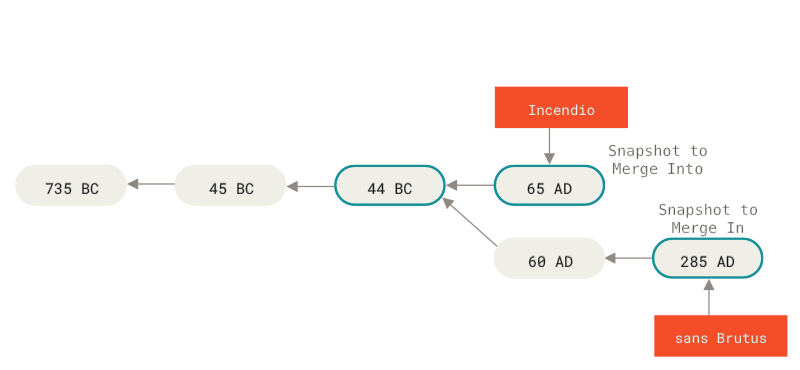
\includegraphics{figs/timeline4.png}

\subsection{}

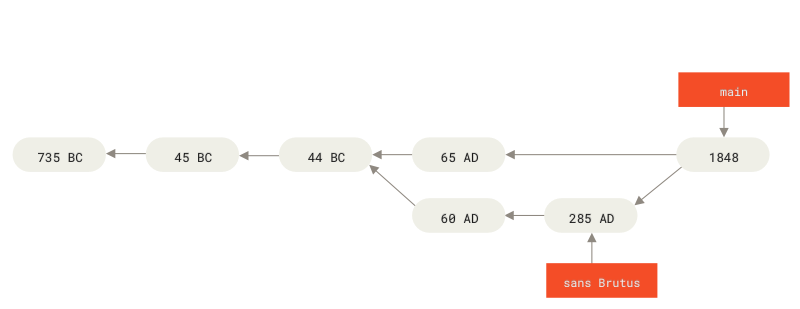
\includegraphics{figs/timeline5.png}

\section{Creando ramas}

El comando para crear nuevas ramas es

\begin{lstlisting}
$ git branch <branchname>
\end{lstlisting}

El crear nuevas ramas implica solamente crear un nuevo apuntador, no se
mueve a una.

. . .

El apuntador especial \passthrough{\lstinline!HEAD!} indica a Git en qué
punto se está trabajando en un momento dado.

\subsection{}

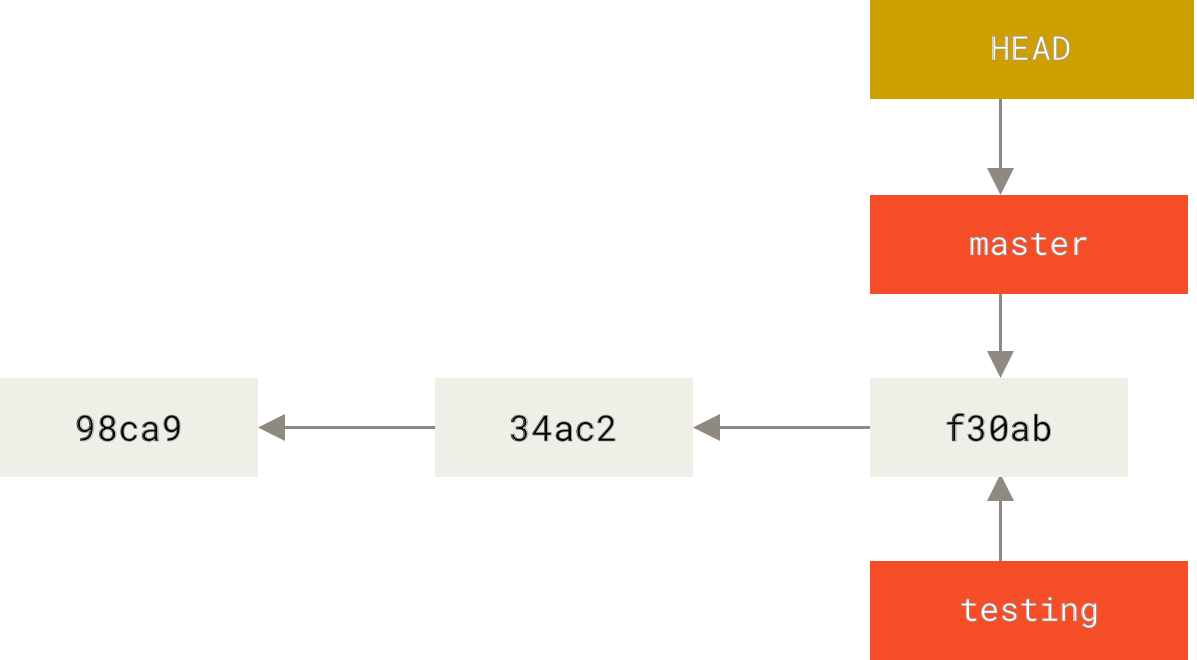
\includegraphics{figs/head-to-master.png}

\subsection{Moviéndonos a otra rama}

Para cambiar de rama, es decir mover el apuntador
\passthrough{\lstinline!HEAD!} para apuntar a
\passthrough{\lstinline!testing!} y empezar a hacer \emph{commit} ahi,
usamos el comando

\begin{lstlisting}
$ git checkout <branch>
\end{lstlisting}

\section{Basic Branching and Merging}

Para unir dos ramas:

\begin{enumerate}
\def\labelenumi{\arabic{enumi}.}
\tightlist
\item
  Checkout la rama receptora
\item
  \passthrough{\lstinline!git merge <branch>!}
\item
  Borrar \passthrough{\lstinline!<branch>!} (opcional)
\end{enumerate}

\section{Merge conflicts}

Cuando intentas unir dos ramas con cambios divergentes, o a la que se
intenta unir no es ancestro directo de la que se une, Git no puede hacer
una unión \emph{fast-forward}. En esos casos, Git tiene que hacer una
unión entre tres commits (\emph{three-way merge}), que podemos pensar
como nodos sobre las ramas. Sin embargo, como los cambios en ambas ramas
no conflictúan entre sí, Git aún puede hacer una unión simple; es decir,
una que no requiere intervención del usuario. Cuando esto sucede, se
dice que no hay conflictos. En este caso particular, la unión se hace
entre los dos nodos usuales más un tercer nodo que es su ancestro común
más cercano.

Al unir dos ramas, Git combina los contenidos de manera automática (si
puede), y automáticamente crea un nuevo \emph{commit}.

\subsubsection{Basic Merge Conflicts}

Hay ocasiones en las que Git no puede hacer uniones simples y necesita
consultar con un usuario cuales cambios mantener. Estos conflictos se
dan cuando se intentan fusionar (unir) dos ramas que tienen cambios que
no son compatibles entre si. Por ejemplo, cuando se modifica un archivo
de dos maneras distintas en el mismo lugar con respecto a el ancestro en
común más cercano.

Un ejemplo de cuando no se puede hacer una unión limpia:

\begin{lstlisting}
$ git merge iss53
Auto-merging index.html
CONFLICT (content): Merge conflict in index.html
Automatic merge failed; fix conflicts and then commit the result.
\end{lstlisting}

Cuando sucede un conflicto, Git pausa el proceso de unión que culmina
con un \emph{commit} y espera a que el usuario resuelva los conflictos.
Si corremos \passthrough{\lstinline!git status!} después de un
conflicto, podemos ver en qué archivos se dió el conflicto para empezar
a solucionarlo

\begin{lstlisting}
$git status
On branch master
You have unmerged paths.
  (fix conflicts and run "git commit")

Unmerged paths:
  (use "git add <file>..." to mark resolution)

    both modified:      index.html

no changes added to commit (use "git add" and/or "git commit -a")
\end{lstlisting}

En el ejemplo anterior el conflicto se dió en el archivo
\passthrough{\lstinline!index.html!}. Cuando ocurre un conflicto Git
modifica los archivos y les añade marcadores para ayudar a resolver el
conflicto. Estos marcadores están para que se pueda abrir manualmente el
archivo, y decidir qué cambios se quedan y cuales se van. Abriendo el
archivo con conflicto, se vería algo como esto:

\begin{lstlisting}
<<<<<<< HEAD:archivo.txt
Contenido en HEAD. Es decir, rama local hacia la cual se hace la union
=======
Contenido en branch, rama que esta siendo unida a HEAD
>>>>>>> branchname:archivo.txt
\end{lstlisting}

Entre los corchetes de apertura \passthrough{\lstinline!<<<<<<<!} y el
separador \passthrough{\lstinline!=======!} están los cambios que están
en donde actualmente se encuentra \passthrough{\lstinline!HEAD!}. Es
decir, los cambios en la rama que está activada actualmente, hacia la
cual se quiere unir. En el encabezado se aclara en qué rama está, y el
archivo que tuvo conflictos. En la parte desde el separador hasta los
corchetes de cerradura \passthrough{\lstinline!>>>>>>>!} están los
cambios \emph{incoming}. Es decir, los que están en la rama que se está
tratando de unir.

Algunos editores de texto y IDEs están configurados para reconocer estos
bloques generados automáticamente por Git, y dan ayuda visual
poniendolos en fondos de colores, o dando botones de ayuda para aceptar
cambios \emph{incoming}, mantener el estado actual, o incluso mantener
ambos. Si tu editor o IDE no tiene esta funcionalidad, puedes usar las
herramientas visuales que vienen con Git, corriendo
\passthrough{\lstinline!git mergetool!}.

Para resolver un conflicto se eligen los cambios a mantener (o se borran
ambos), y se quitan los marcadores generados por Git. Una vez que se
decidió qué cambios mantener y se añade el archivo resuelto (sin
marcadores) al \emph{Staging Area}, Git entenderá que el conflicto fue
resuelto. Si se corre \passthrough{\lstinline!git status!} en este punto
Git pedirá confirmación de que se resolvió exitosamente el conflicto.
Para finalizar la unión se confirman todos los cambios con
\passthrough{\lstinline!git commit!}. Nótese que ahora no escribimos un
mensaje de confirmación, Git lo añade automáticamente con la información
más importante para señalizar que hubo una unión y resolución de
conflicto.

\subsubsection{Branch Management}

El comando \passthrough{\lstinline!git branch!} al usarse sin argumentos
va a listar todas las ramas del repo, y marca la activa con un
\passthrough{\lstinline!*!} al lado izquierdo de su nombre. Para mostrar
el \emph{commit} más reciente en cada rama, se puede usar
\passthrough{\lstinline!git branch -v!}.

A veces es util ver si las ramas tienen cambios incorporados a la rama
actual, o si aún no se han unido. Para esto existen las opciones
\passthrough{\lstinline!–merged!} y \passthrough{\lstinline!–no-merged!}
que actúan como filtro. Por ejemplo al correr

\begin{lstlisting}
$ git branch --merged
  mergedbranch
* master
\end{lstlisting}

vemos que la rama \passthrough{\lstinline!mergedbranch!} ya fué unida a
\passthrough{\lstinline!master!}. Como ya está unida, es seguro
eliminarla con \passthrough{\lstinline!git branch -d mergedbranch!} sin
ningún peligro. Sin embargo, si intentamos eliminar una rama que no ha
sido unida, digamos \passthrough{\lstinline!unmerged-b!}, Git nos dará
un error y pedirá confirmación.

\begin{lstlisting}
$ git branch -d unmerged-b
error: The branch 'unmerged-b' is not fully merged.
If you are sure you want to delete it, run 'git branch -D unmerged-b'.
\end{lstlisting}

Como muestra el mensaje de ayuda del comando anterior, se puede
sobreescribir el mecanismo de Git diseñado para no perder cambios usando
el switch \passthrough{\lstinline!-D!} (en mayúscula). Esto solo se hace
si estás consciente de que se perderán todos los cambios en esa rama.
Por ejemplo, si era una rama \emph{throwaway} en la que se hizo un
experimento. \# Basic Branching and Merging

El procedimiento básico para unir (\emph{merge}) dos ramas es moverse, o
``activar'' (\emph{checkout}) la rama hacia la cual se va a unir, y
correr el comando \passthrough{\lstinline!git merge <branch>!}. Hay
diferentes tipos de \emph{merge}s que pueden ocurrir. Cuando la rama que
se unió estába directamente adelante, sin cambios divergentes, Git lleva
a cabo una unión \emph{fast-forward} (avance rápido). Es decir, Git
simplemente mueve el apuntador \passthrough{\lstinline!HEAD!} hacia
adelante.

Si después de unir dos ramas ya no necesitas la que fue unida, la puedes
eliminar fácilmente con el comando \passthrough{\lstinline!branch!} y la
opción \passthrough{\lstinline!-d!}, corto para
\passthrough{\lstinline!–delete!}

\begin{lstlisting}
$ git branch -d <branch>
\end{lstlisting}

Cuando intentas unir dos ramas con cambios divergentes, o a la que se
intenta unir no es ancestro directo de la que se une, Git no puede hacer
una unión \emph{fast-forward}. En esos casos, Git tiene que hacer una
unión entre tres commits (\emph{three-way merge}), que podemos pensar
como nodos sobre las ramas. Sin embargo, como los cambios en ambas ramas
no conflictúan entre sí, Git aún puede hacer una unión simple; es decir,
una que no requiere intervención del usuario. Cuando esto sucede, se
dice que no hay conflictos. En este caso particular, la unión se hace
entre los dos nodos usuales más un tercer nodo que es su ancestro común
más cercano.

Al unir dos ramas, Git combina los contenidos de manera automática (si
puede), y automáticamente crea un nuevo \emph{commit}.

\subsubsection{Basic Merge Conflicts}

Hay ocasiones en las que Git no puede hacer uniones simples y necesita
consultar con un usuario cuales cambios mantener. Estos conflictos se
dan cuando se intentan fusionar (unir) dos ramas que tienen cambios que
no son compatibles entre si. Por ejemplo, cuando se modifica un archivo
de dos maneras distintas en el mismo lugar con respecto a el ancestro en
común más cercano.

Un ejemplo de cuando no se puede hacer una unión limpia:

\begin{lstlisting}
$ git merge iss53
Auto-merging index.html
CONFLICT (content): Merge conflict in index.html
Automatic merge failed; fix conflicts and then commit the result.
\end{lstlisting}

Cuando sucede un conflicto, Git pausa el proceso de unión que culmina
con un \emph{commit} y espera a que el usuario resuelva los conflictos.
Si corremos \passthrough{\lstinline!git status!} después de un
conflicto, podemos ver en qué archivos se dió el conflicto para empezar
a solucionarlo

\begin{lstlisting}
$git status
On branch master
You have unmerged paths.
  (fix conflicts and run "git commit")

Unmerged paths:
  (use "git add <file>..." to mark resolution)

    both modified:      index.html

no changes added to commit (use "git add" and/or "git commit -a")
\end{lstlisting}

En el ejemplo anterior el conflicto se dió en el archivo
\passthrough{\lstinline!index.html!}. Cuando ocurre un conflicto Git
modifica los archivos y les añade marcadores para ayudar a resolver el
conflicto. Estos marcadores están para que se pueda abrir manualmente el
archivo, y decidir qué cambios se quedan y cuales se van. Abriendo el
archivo con conflicto, se vería algo como esto:

\begin{lstlisting}
<<<<<<< HEAD:archivo.txt
Contenido en HEAD. Es decir, rama local hacia la cual se hace la union
=======
Contenido en branch, rama que esta siendo unida a HEAD
>>>>>>> branchname:archivo.txt
\end{lstlisting}

Entre los corchetes de apertura \passthrough{\lstinline!<<<<<<<!} y el
separador \passthrough{\lstinline!=======!} están los cambios que están
en donde actualmente se encuentra \passthrough{\lstinline!HEAD!}. Es
decir, los cambios en la rama que está activada actualmente, hacia la
cual se quiere unir. En el encabezado se aclara en qué rama está, y el
archivo que tuvo conflictos. En la parte desde el separador hasta los
corchetes de cerradura \passthrough{\lstinline!>>>>>>>!} están los
cambios \emph{incoming}. Es decir, los que están en la rama que se está
tratando de unir.

Algunos editores de texto y IDEs están configurados para reconocer estos
bloques generados automáticamente por Git, y dan ayuda visual
poniendolos en fondos de colores, o dando botones de ayuda para aceptar
cambios \emph{incoming}, mantener el estado actual, o incluso mantener
ambos. Si tu editor o IDE no tiene esta funcionalidad, puedes usar las
herramientas visuales que vienen con Git, corriendo
\passthrough{\lstinline!git mergetool!}.

Para resolver un conflicto se eligen los cambios a mantener (o se borran
ambos), y se quitan los marcadores generados por Git. Una vez que se
decidió qué cambios mantener y se añade el archivo resuelto (sin
marcadores) al \emph{Staging Area}, Git entenderá que el conflicto fue
resuelto. Si se corre \passthrough{\lstinline!git status!} en este punto
Git pedirá confirmación de que se resolvió exitosamente el conflicto.
Para finalizar la unión se confirman todos los cambios con
\passthrough{\lstinline!git commit!}. Nótese que ahora no escribimos un
mensaje de confirmación, Git lo añade automáticamente con la información
más importante para señalizar que hubo una unión y resolución de
conflicto.

\subsubsection{Branch Management}

El comando \passthrough{\lstinline!git branch!} al usarse sin argumentos
va a listar todas las ramas del repo, y marca la activa con un
\passthrough{\lstinline!*!} al lado izquierdo de su nombre. Para mostrar
el \emph{commit} más reciente en cada rama, se puede usar
\passthrough{\lstinline!git branch -v!}.

A veces es util ver si las ramas tienen cambios incorporados a la rama
actual, o si aún no se han unido. Para esto existen las opciones
\passthrough{\lstinline!–merged!} y \passthrough{\lstinline!–no-merged!}
que actúan como filtro. Por ejemplo al correr

\begin{lstlisting}
$ git branch --merged
  mergedbranch
* master
\end{lstlisting}

vemos que la rama \passthrough{\lstinline!mergedbranch!} ya fué unida a
\passthrough{\lstinline!master!}. Como ya está unida, es seguro
eliminarla con \passthrough{\lstinline!git branch -d mergedbranch!} sin
ningún peligro. Sin embargo, si intentamos eliminar una rama que no ha
sido unida, digamos \passthrough{\lstinline!unmerged-b!}, Git nos dará
un error y pedirá confirmación.

\begin{lstlisting}
$ git branch -d unmerged-b
error: The branch 'unmerged-b' is not fully merged.
If you are sure you want to delete it, run 'git branch -D unmerged-b'.
\end{lstlisting}

Como muestra el mensaje de ayuda del comando anterior, se puede
sobreescribir el mecanismo de Git diseñado para no perder cambios usando
el switch \passthrough{\lstinline!-D!} (en mayúscula). Esto solo se hace
si estás consciente de que se perderán todos los cambios en esa rama.
Por ejemplo, si era una rama \emph{throwaway} en la que se hizo un
experimento. \# Branching Workflows

En esta subsección revisamos algunos de los \emph{workflows} más comunes
que se usan para trabajar con Git y ramas. Esto es en realidad más
descriptivo que normativo, pero es útil para estructurar proyectos
grandes. En especial porque estos \emph{workflows} están diseñados para
evitar conflictos a la hora de las uniones, y tener tantas uniones
simples como sea posible.

\subsubsection{Long-Running Branches}

La estructura de desarrollo de ramas \emph{long-running} se basa en
tener un número pequeño de ramas principales que siempre están abiertas,
dedicadas a las diferentes etapas del desarrollo, las cuales se unen
entre si de manera regular.

Una estrategia común es tener dos ramas principales: \emph{master} y
\emph{development} (los nombres no son importantes). En
\passthrough{\lstinline!master!} se tiene el código en su estado más
pulido, mientras que en \passthrough{\lstinline!development!} se hacen
los cambios importantes que solo se unen a
\passthrough{\lstinline!master!} una vez que están terminados, probados,
etc\ldots{} Es usual agregar una rama o serie de ramas más dedicadas a
resolver problemas particulares. Estas ramas se unen a
\passthrough{\lstinline!development!} una vez que se resolvió aquello
para lo cual fueron creadas, y se eliminan poco después. Este tipo de
ramas se conocen como \emph{topic branches}, o ramas de tema.

Es útil pensar en las ramas estructuradas de esta manera como almacenes
en los que se guarda código en función de su madurez. \# Rebasing

Como el nombre sugiere, consiste en cambiar de base una versión
particular. Es decir, es como hacer los cambios que se efectuaron a
través de una rama, como si se hubieran hecho empezando desde otro punto
de la rama o de otra rama por completo.

\begin{lstlisting}
$ git rebase master
\end{lstlisting}

La operación funciona encontrando al ancestro común de las dos ramas que
se están uniendo, y aplicando lo cambios gradualmente. Una vez que se
hace un \emph{rebase}, se puede hacer un \emph{merge} simple del tipo
\emph{fast-forward} hasta la punta de la rama. Todo eso gracias a que
ahora la punta de la rama y el \emph{commit} al que se hizo el
\emph{rebase} tienen una ancestría en común, una ancestría lineal. Ya no
hay ningún conflicto de versiones.

Vale la pena hacer notar que el producto final no tiene nada de
diferente a hacer un \emph{merge}. La única ventaja notable es que hace
que la historia de \emph{commits}, los logs, esté más limpio y claro.

Hay \emph{rebases} más complejos, pero francamente no entendí del todo,
y valdrá la pena revisarlo con más calma.

\subsubsection{No incluí los cambios que quería en un commit anterior.
¿Ahora qué hago?}

Ua buena aplicación del rebasing es justo en la situación del título.
¿Qué tal si yo tenía planeado incluir los cambios a el archivo
\passthrough{\lstinline!ìndex.txt!} en un commit que hice con el mensaje
``Cambios a index.txt'', pero me equivoqué y no añadí
\passthrough{\lstinline!index.txt!} al \emph{staging area} antes de ese
commit?

En concreto: Consideremos el log de cambios de un repo:

\begin{lstlisting}
a0b0c0E3 (HEAD -> master) Cambios que no eran de index.txt
.
.
.
a0b0c0E1 Cambios a index.txt
\end{lstlisting}

Digamos que yo quería incluir los cambios a
\passthrough{\lstinline!index.txt!} en el commit con hash
\passthrough{\lstinline!a0b0c0E1!}, pero al correr
\passthrough{\lstinline!git status!} me señala que los cambios no están
``staged for commit'' para el siguiente commit y por lo tanto no se
añadieron antes. Para volver a antes de
\passthrough{\lstinline!a0b0c0E1!} y ahora si añadir los cambios en ese
commit, podemos usar rebase como en la siguiente receta:

\begin{enumerate}
\def\labelenumi{\arabic{enumi}.}
\item
  \passthrough{\lstinline!git rebase –interactive ’a0b0c0E1\^’!}. Nótese
  que el hash del commit al que nos estamos refiriendo está postfijo por
  un ``caret'' (\^{}). Eso indica rebase no a
  \passthrough{\lstinline!a0b0c0E1!}, sino \emph{antes} de el.
\item
  En el editor predeterminado se abrirá un archivo que se ve más o menos
  asi:

\begin{lstlisting}
pick a0b0c0E3 HEAD Cambios que no eran de index.txt
pick a0b0c0E1 Cambios a index.txt
\end{lstlisting}

  Cambia \passthrough{\lstinline!pick!} a \passthrough{\lstinline!edit!}
  en la línea que tiene el chash del commit el cual deseas modificar o
  añadirle archivos. Guarda el archivo y ciérralo.
\item
  Después de los pasos anteriores, Git marca al commit
  \passthrough{\lstinline!a0b0c0E1!} como el actual (donde se encuentra
  \passthrough{\lstinline!HEAD!}), y por lo tanto se le pueden añadir
  cambios con ammend. Por ejemplo:

\begin{lstlisting}
git add index.txt
git commit --amend -m "Ahora si, cambios a index.txt"
\end{lstlisting}
\item
  Para acabar y volver a la punta de la rama actual, es decir donde
  estábamos antes, seguimos el consejo de Git y corremos
  \passthrough{\lstinline!git rebase     –continue!}.\# Distributed
  workflows
\end{enumerate}
